\documentclass[twocolumn]{revtex4-2}
\usepackage{graphicx}
\usepackage{amsmath}
\usepackage{amsthm}
\usepackage{amssymb}
\usepackage{physics}
\usepackage{hyperref}
\usepackage{tikz-cd}
\usepackage{hvfloat}
\usepackage{float}

\newtheorem{definition}{Definition}
\newtheorem{proposition}{Proposition}
\newtheorem{theorem}{Theorem}
\newtheorem{lemma}{Lemma}
\newtheorem{corollary}{Corollary}
\bibliographystyle{plain}
\DeclareMathOperator*{\maximize}{maximize}


\begin{document}
\title{Padé Partial Dual Method for Finding Bounds in Inverse Design}
\author{Justin Cardona}
\affiliation{Engineering Physics Department, Polytechnique Montréal}
\begin{abstract}
This work presents a method for forming Lagrange Dual for Inverse Design programs that circumvents the need to check for positive definiteness during optimization. By using a Partial Dual approach and leveraging compact constraints, this problem is replaced with a root finding task that is typically solved here in three iterations using Padé approximations, regardless of system size. The solution is used to efficiently shift the Lagrangian of the system to positive definiteness.
\end{abstract}
\maketitle

\section{Introduction}
\label{sec:intro}
Inverse design is the idea of automating the engineering process to algorithmically find designs that outperform human intuition. There have been several examples of this approach surpassing the state of the art for many important applications such as radiative Purcell enhancement \cite{molesky2020hierarchical}, metamaterial photonics \cite{shen2014ultra}, solar energy \cite{ganapati2013light}, and non-linear switching \cite{elesin2012design} for example. This is typically done by phrasing the creation of an optical device as a mathematical optimization problem and finding its solution. The issue is that these problems are non-convex in general so little inverse design literature can make claims about the global optimality of the designs that are produced.

In addition to this uncertainty, current designs are restricted to very few degrees of freedom. These are highly specialized problems that have high degrees of symmetry or are not even three dimensional, typically having low resolution. There have been some 3D results, but only for sub-wavelength problems (see \cite{xue2023fullwave} for example). This is due to the fact that many of the numerical tasks to be performed scale poorly with the degrees of freedom.
\subsection{Electromagnetics Notation}
\label{sec:notation}
In order to discuss the goal of this thesis more fully, a framework to describe electromagnetics will first be presented. Consider the set of square integrable complex fields in 3D real space $L^2(\mathbb{R}^3, \mathbb{C}^6)$ with the inner product:

\begin{align}
\braket{F}{G} = \int_{\mathbb{R}^3}&d^3xF(x)^*\cdot G(x)\\
&\forall \ket{F}, \ket{G}\in L^2(\mathbb{R}^3, \mathbb{C}^6)\nonumber
\end{align}
Using this, one may write Maxwell's equations as:

\begin{align}
\mu_0\partial_t\qty(\ket{H} + \ket{m}) + \curl\ket{E} &= 0\\
\epsilon\partial_t\ket{E} - \curl\ket{H} &= -\ket{J}.\nonumber
\end{align}
Fourier transforming in time, they can be written in matrix form as:

\begin{align}
\mqty(\ket{J} \\-\ket{m}) = \mqty(-i\epsilon\omega & \curl \\ \frac{i}{\mu_0\omega}\curl & 1)\mqty(\ket{E}\\\ket{H}).
\end{align}
Using magnetic currents instead allows for a cleaner representation and a hermitian matrix. Letting $\ket{M}=\mu_0\partial_t\ket{m}$, $Z = \sqrt{\frac{\mu_0}{\epsilon}}$, and $k = \sqrt{\mu_0\epsilon}$:

\begin{align}
\frac{i}{k}\mqty(\ket{J} \\-\ket{M}) = -\mqty(Z^{-1} & -\frac{i}{k}\curl \\ \frac{i}{k}\curl & Z)\mqty(\ket{E}\\\ket{H}).
\end{align}

Concatenating the currents and field together, the above expression may be written as $\frac{i}{k}\ket{p}=M\ket{f}$. Additionally, $M_0$, in place of $M$, will refer to the Maxwell operator of \textit{free space}. The permeability and permittivity response function will be denoted $X\in \text{GL}\qty(L^2\qty(\mathbb{R}^3,\mathbb{C}^6))$, breaking this up into the electric and magnetic components, this relates currents with fields in the typical sense, $\frac{i}{k}\ket{p^s}=-X\ket{f}$, or

\begin{align}
\frac{i}{k}\mqty(\ket{J^s}\\-\ket{M}) = -\mqty(z^{-1}X_{JE} & X_{JH}\\ z^{-1}X_{ME} & X_{MH})\mqty(\ket{E}\\\ket{H}).
\end{align}
Here, $z=\sqrt{\mu_0/\epsilon_0}$ while $i$ and $s$ superscripts denote incident and scattered fields so that any total field may be written $g = g^i + g^s$. This allows Maxwell's equations in a medium to be written as

\begin{align}
-\frac{i}{k}\ket{p^i} = \qty(M_0-X)\ket{f}.
\end{align}
Instead opting to use the Green's function operator (for free space) $G_0$, Maxwell's equations are:

\begin{align}
-\frac{i}{k}\qty(X^{-1}-G_0)\ket{p^s}=\ket{f^i}.
\end{align}
Denoting the source field as $\ket{S} = ik\ket{f^i}$ and the transmitted currents $\ket{T} = \ket{p^s}$, Maxwell's equations imply:

\begin{align}
\braket{S}{T} = \ev{U}{T}.
\label{eq:power_transfer}
\end{align}
with $U=X^{-\dagger}-G_0^\dagger$. The idea behind using currents rather than fields is that it, combined with an integral formalism presents better numerical convergence \cite{markkanen2012discretization}.

\subsection{Inverse Design Context}
\label{sec:context}
The goal of inverse design is to automatedly create optical devices. This is done by phrasing the design process as a mathematical optimization problem with an objective function that captures the goal of the project (to be maximized). The design variable is the optical device itself. In other words, one finds the best way of arranging material in physical space in order to achieve the best possible outcome. Mathematically this is the program

\begin{align}
	\maximize_{X\in\text{GL}\qty(L^2\qty(\mathbb{R}^3, \mathbb{C}^6))} f\qty(X)
\end{align}
where $f:\text{GL}\qty(L^2\qty(\mathbb{R}^3, \mathbb{C}^6))\rightarrow\mathbb{R}$. Many important problems in photonics can be represented by net-power-transfer objectives \cite{molesky2020global}. These take on the following form

\begin{align}
	\maximize_{X\in\text{GL}\qty(L^2\qty(\mathbb{R}^3, \mathbb{C}^6))} \Im\braket{S}{T} - \ev{Q}{T}
\end{align}
where $Q$ is introduced for a general quadratic form. For example, $Q=\text{ASym}G_0$ for absorption/material loss problems, $\text{ASym}X^{-\dagger}$ for scattering/radiation, or $0$ for extracted power\cite{molesky2020global}. In these problems, one is given a source field $\ket{S}$ and an $X$ is found such that the transmitted current $\ket{T}$ has the desires properties. It should be noted that in practice materials have highly localized response, so $X$ is nearly diagonal and is approximated as such. This allows for an easy invertible map between $X$ and $\ket{T}$, namely $\ket{T} = X\qty(\ket{S}, G_0\ket{T})$. Therefore, given $\ket{S}$ and $\ket{T}$, $X$ can be found via element-wise division. This greatly simplifies the problem because now one can have a fixed $X$ and treat $\ket{T}$ as the optimization variable in a quadratic program. The tradeoff here is that Maxwell's equations must now be enforced explicitly through equation \ref{eq:power_transfer}. This problem will be addressed along with discretization.

When actually computing a design, one does not solve for the physical field but rather a discretization of it. For a design region $\mathcal{R}$, one may consider a collection of subsets $R$. The elements of $R$ are convex and span $\mathcal{R}$. These cells usually lie on a cubic lattice, but for generality an abstract $R$ will do fine. Consider the discretization operator $\delta:L^2(\mathbb{R}^3, \mathbb{C}^6)\rightarrow\qty(R\rightarrow\mathbb{C}^6)$ such that $(\delta\ket{f})(r) = \ket{f}(\bar{r})$. This is well defined because the centroid $\bar{r}\in\mathcal{R}\subset\mathbb{R}^3$. Similarly for operators $\Delta:\text{GL}\qty(L^2(\mathbb{R}^3, \mathbb{C}^6))\rightarrow\text{GL}\qty(R\rightarrow\mathbb{C}^6)$, the evaluation happens as $(\Delta G)(\ket{f})(r)=G\ket{f}(\bar{r})$. Now for a final note on how to enforce Maxwell's equations. The simplest way is to say that $\forall r\in R$ equation \ref{eq:power_transfer} holds. However, for computational efficiency, it might be sufficient to consider a partitioning set of connected subsections of $R$, $\Omega_R$ and impose \cite{molesky2020hierarchical}:

\begin{align}
	\forall \omega\in\Omega_R \mel{S}{\mathbb{I}_\omega}{T} = \ev{U\mathbb{I}_\omega}{T}
\end{align}
With this in mind, note that further discussion will occur in the discretized context. That is to say that there is a change of variables occuring: $\ket{T}\rightarrow\delta\ket{T}$, $Q\rightarrow\Delta Q$, etc. The fully discretized optimization problem may then be written as

\begin{align}
	\label{eq:opt_exact}
	\text{P}=&\maximize_{\ket{T}\in R\rightarrow\mathbb{C}^6}\qquad\qquad \Im\braket{S}{T} - \ev{Q}{T}\\
	&\text{such that } \forall \omega\in\Omega_R \mel{S}{\mathbb{I}_\omega}{T} = \ev{U\mathbb{I}_\omega}{T}\nonumber
\end{align}
The goal is ultimately to efficiently find globally optimal solutions to the above program when the number of elements in $R$ is very large. In general, it may be difficult to find the global optima as the problem is not convex. However, by using Lagrange duality it is always possible to find a convex optimization problem that yields an upper bound on design performance. Therefore it is very important to be able to solve this problem.

\subsection{Lagrange Duality}
\label{sec:lagrange_duality}
In order to have further insight into this problem, an overview of some key ideas of Lagrange duality will be presented. Consider the following program:

\begin{align}
	\label{eq:primal_general}
	\text{P}=&\maximize_{x\in\mathbb{C}^n} f_0(x)\\
	&\text{such that } \forall m\in\qty{1, \dots M}f_m\ge 0\nonumber.
\end{align}
where $\forall m\in\qty{0, \dots M}$ $f_m:\mathbb{C}^n\rightarrow\mathbb{R}$. This can alternatively be represented as an unconstrained optimization through the use of indicator functions.

\begin{align}
	\text{P}=&\maximize_{x\in\mathbb{C}^n} f_0(x) + \sum_{m=1}^M\mathbb{I}\qty(f_m(x)\ge 0)
\end{align}
where the indicators are defined as:
\begin{align}
	\mathbb{I}(x) = \begin{cases}0 &\text{ if $x$ is true}\\-\infty &\text{ if $x$ is false}\end{cases}
\end{align}
The discontinuous nature of this objective makes it impractical to use gradient methods to find a solution. Therefore, instead of using indicators one can use a linear barrier function with positive coefficients. This will reward a positive value for the constraint function while penalizing negative values.

\begin{align}
	\maximize_{x\in\mathbb{C}^n} f_0(x) + \sum_{m=1}^M \lambda_mf_m(x)
\end{align}
The tradeoff for this continuous form is that the reward terms now add a non-zero portion to the objective. However, if $x$ is in the feasible set $F_\text{P}$ (it satisfies the constraints), then this is still an upper bound. $\mathcal{L}(x, \lambda) = f_0(x) + \sum_{m=1}^M \lambda_mf_m(x)$ is referred to as the Lagrangian, and $\mathcal{D}(\lambda) = \sup_{x\in\mathbb{C}^N}\mathcal{L}(x, \lambda)$ is the dual function. In order to find the best lower bound, one can minimize the dual function. This results in the dual program:

\begin{align}
\text{D}(\text{P}) = \inf_{\lambda\in\mathbb{R}^M_{\ge}}\sup_{x\in\mathbb{C}^N}\mathcal{L}(x, \lambda)
\end{align}

Note that this problem is convex in the Lagrange multipliers. Furthermore, note that for any feasible $x$, $\mathcal{L}$ is an upper bound to $f_0$. Since the constraints are satisfied, the $f_m$ terms can only increase the value of the function. The dual approach is valuable for this reason: it is a convex problem that bounds the primal one. Therefore standard optimization methods can be used to guarantee a bound on the performance of any design.

\section{Duality in Nanophotonics}
\label{sec:duality_in_nanophotonics}
Returning to equation \ref{eq:opt_exact}, for the sake of the computational context, instead of working on $R\rightarrow\mathbb{C}^6$, since $R$ is finite, the space $\mathbb{C}^N$ will be used with $N=6|R|$. Similarly $Q, U, \dots$ can be represented by matrices in $\mathbb{C}^{N\times N}$. 

\begin{align}
	\label{eq:opt_discrete}
	\text{P}=&\maximize_{\ket{T}\in \mathbb{C}^N}\qquad\qquad \Im\braket{S}{T} - \ev{Q}{T}\\
	&\text{such that } \forall \omega\in\Omega_R \mel{S}{\mathbb{I}_\omega}{T} = \ev{U\mathbb{I}_\omega}{T}\nonumber
\end{align}
One may note that the Hermitian and anti-Hermitian parts of the equation  hold independently and thus can be separated into two constraints.  The tendency of this optimization is to increase the magnitude of $\ket{T}$. Therefore the only side of the equalities that ends up being enforced are the "$\ge$" ones as they provide an upper bound to the norm of $\ket{T}$ :
\begin{align}
	\label{eq:opt_ineq}
	\text{P}=\maximize_{\ket{T}\in \mathbb{C}^N} &\Im\braket{S}{T} - \ev{Q}{T}\\
	\text{such that } \forall &\omega\in\Omega_R \Im\mel{S}{\mathbb{I}_\omega}{T} \ge \ev{\text{Asym}\qty(U\mathbb{I}_\omega)}{T}\nonumber\\
	&\qquad\quad\ \Re\mel{S}{\mathbb{I}_\omega}{T} \ge \ev{\text{Sym}\qty(U\mathbb{I}_\omega)}{T}\nonumber
\end{align}

 Now that the problem has been properly stated, it is time to begin finding the dual problem. The goal of this is to obtain a convex optimization problem that can be solved using standard gradient methods in order to give a bound on the primal. The Lagrangian of this program is:

 \begin{align}
	\mathcal{L} &= \Im\braket{S}{T} - \ev{Q}{T}\\
	&+ \sum_{m=1}^M \alpha_m\qty(\Re\mel{S}{\mathbb{I}_\omega}{T} - \ev{\text{Sym}\qty(U\mathbb{I}_\omega)}{T})\nonumber\\
	&+ \sum_{m=1}^M \beta_m\qty(\Im\mel{S}{\mathbb{I}_\omega}{T} - \ev{\text{ASym}\qty(U\mathbb{I}_\omega)}{T})\nonumber
 \end{align}
but here M= $|\Omega_R|$ and $\mathbb{I}_m$  is the projection onto the $m^\text{th}$ element of $\Omega_R$.

\begin{align}
	\mathcal{L} &= \mqty(\bra{T} & \bra{S})\mqty(-L_{TT} & T_{TS} \\ L_{TS}^\dagger & 0)\mqty(\ket{T} \\ \ket{S})\\
	L_{TT} &=  Q + \sum_{m=1}^M (\alpha_m\ev{\text{Sym}\qty(U\mathbb{I}_\omega)}{T}\nonumber\\
	&\qquad +\beta_m\ev{\text{ASym}\qty(U\mathbb{I}_\omega)}{T})\nonumber\\
	L_{TS} &=  \frac{1}{2i}\mathbb{I} + \frac{1}{2}\sum_{m=1}^M \qty(\alpha_m + i\beta_m)\mathbb{I}_m\nonumber
\end{align}
In order for the dual to give a meaningful bound on the primal, $L=\mqty(-L_{TT} & L_{TS}\\ L_{TS}^\dagger & 0)\succcurlyeq 0$ is needed. This requires that $L_TT\succcurlyeq 0$.

\subsection{Dual Numerical Difficulties}
\label{sec:dual_numerical_difficulties}
In order to show whether the matrix is positive definite, one of two approaches is typically done. The first is by checking whether the Cholesky decomposition terminates \cite{roux2016formal, rump2006verification}. Given a matrix $A\in\mathbb{C}^{N\times N}$, a Cholesky decomposition is when A can be written as $LL^\dagger$  where $L$ a triangular matrix with real and positive diagonal entries.  It is a necessary and sufficient condition \cite{schnabel1990new}. The issue is that the discretization of the design region may contain potentially millions of cells (elements of $R$), so Cholesky decomposing $L_{TT}$ is completely impractical given its cubic scaling \cite{trefethen2022numerical}. For this reason it is unfeasible, especially in the case of large-scale inverse design.

An alternative approach that is commonly used are randomized trace estimators for log barrier methods \cite{boyd2004convex}. The most performant and generally applicable method is the Hutchinson trace estimator, these work in the following way. Assume it is known that the matrix is initially positive definite (known and by doing a costly method). Each time the Lagrange multipliers are updated, it must be verified whether the matrix is still positive definite. Since the multipliers undergo very small changes, and the eigenvalues have a continuous dependence on them (from the characteristic equation), one might intuitively expect that the eigenvalues of $L_{TT}$ will become vanishing small before they become negative. One can test for this case by evaluating $\log\det L_{TT}$. This is due to the fact that $\det L_{TT}=\prod_{n=1}^N\lambda_n$, the product of $L_{TT}$’s eigenvalues. This means $\log\det L_{TT}=\sum_{n=1}^N\log\lambda_n$. Note that when $\lambda_n\rightarrow 0$ $\log\lambda_n\rightarrow-\infty$ so when $\log\det L_{TT}$ is large and negative, it indicates that $L_{TT}$ is nearly indefinite.

While $\det L_{TT}$ it is very expensive to evaluate, note that

\begin{align}
\log\det L_{TT}=\sum_{n=1}^N\log\lambda_n = \text{Tr}\log L_{TT}
\end{align}
so one could estimate the trace instead of the determinant, which is cheaper. First a series expansion is found:

\begin{align}
\log L_{TT} &= \log(I + \qty(L_{TT} - I))\\
&=\sum_{k=1}^\infty\frac{-1^{k+1}}{k}\qty(L_{TT} - I)^k
\end{align}
and then the trace is evaluated:


\begin{align}
\text{Tr}\log L_{TT} &= \sum_{k=1}^\infty\frac{-1^{k+1}}{k}\text{Tr}\qty(L_{TT} - I)^k
\end{align}
Now, regarding how the trace is efficiently estimated. The Hutchinson trace is defined for $A\in \mathbb{C}^{m\times m}$ as \cite{skorski2021modern}:

\begin{align}
\text{Tr}_{H^n}A = \frac{1}{n}\sum_{i=1}^n \ev{A}{z_i},\quad &z\sim\qty{-1, 1}^m
\end{align}
With probability $1-\delta$ this has a relative error of $\epsilon$, given that $n$ samples have been drawn:

\begin{align}
n = \frac{2}{\epsilon^2}\qty(2+\frac{8\sqrt{2}}{3})\log(\frac{2}{\delta})
\end{align}
There are a few issues with this approach. Firstly, the log expansion has truncation error that compounds with this. Secondly, the series requires $\norm{L_{TT} - I} < 1$ which is not always true. This is usually circumvented by doing $\log A = 2n\log A^{1/2n}$, but square roots are too expensive here. Even assuming complete accuracy in the log, for a 99\% chance of a 0.1\% error 30,460,939 sample matrix vector products are needed. For a 75\% chance of a 1\% error 84,746 matrix vector products are needed.

These methods are very expensive a better alternative will be presented. Recall the Lagrangian of the primal problem \ref{eq:opt_ineq}. In order to circumvent having to check whether $L_{TT}\succ 0$, a compact constraint is singled out and imposed explicitly. Namely, this will be the anti-symmetric constraint over the entire domain. This means making the change $R\rightarrow R\setminus\qty{\mathcal{R}}$ in equation \ref{eq:opt_ineq} in addition to adding the constraint explicitly. Of course D(P) with $\mathcal{D}$ in this form is still dual to P, but this form allows for another manipulation, finding a \textit{partial} dual $\text{D}^\partial(P)$ which has the Lagrangian \cite{molesky2020hierarchical}:

\begin{align}
	\mathcal{L}^\partial &= \mqty(\bra{T} & \bra{S})L\mqty(\ket{T} \\ \ket{S}) + \gamma\qty(\Im\braket{S}{T} - \ev{\text{ASym}U}{T})\nonumber\\
	&=\mqty(\bra{T} & \bra{S})L^\partial\mqty(\ket{T} \\ \ket{S})
\end{align}
Note that this means $L^\partial_{TT} = L_{TT} + \gamma E$, $L^\partial_{TS} = L_{TS} + i\gamma\mathbb{I}$, with $E=\text{Asym} U$. The real potential issue here is $L_{TT}$, but since $E\succ 0$, if $\gamma$ is large enough $L^\partial$ is as well. When this is the case, the optimal value of $\ket{T}$ can be expressed in terms of the Lagrange multipliers by finding stationary points:

\begin{align}
\frac{\partial}{\partial\ket{T}}\mathcal{L}^\partial &= \frac{\partial}{\partial\ket{T}}\qty(-\ev{L^\partial_{TT}}{T} + \mel{T}{L^\partial_{TS}}{S} + \mel{S}{L^{\partial\dagger}_{TS}}{T})\nonumber\\
&\implies L^\partial_{TT}\ket{T} = L^\partial_{TS}\ket{S}
\end{align}
The goal therefore, is to find the smallest partial dual multiplier $\gamma_*$ such that $L_{TT} + \gamma_* E\succcurlyeq 0$ and $C_\gamma =\Im\braket{S}{T_\gamma} - \ev{E}{T_\gamma}\ge 0$. To show that such a solution does exist, consider the derivatives of $C_\gamma$:

\begin{align*}
\frac{dC_\gamma}{d\gamma} &= 2\qty(\frac{1}{2}\bra{S} - i\bra{T_\gamma}E)L^{\partial -1}_{TT}\qty(\frac{1}{2}\ket{S} + iE\ket{T})\\
\frac{d^2C_\gamma}{d\gamma^2} &= -6\qty(\frac{1}{2}\bra{S} - i\bra{T_\gamma}E)L^{\partial -1}_{TT} E L^{\partial -1}_{TT}\qty(\frac{1}{2}\ket{S} + iE\ket{T})
\end{align*}
When $L^\partial_{TT}\ge 0$ then both derivatives are positive and:

\begin{align*}
\lim_{\gamma\rightarrow\infty}C_\gamma = \frac{1}{4}\ev{E^{-1}}{S}
\end{align*}
Therefore there does exist $\gamma_*$ that satisfies the previously stated criteria. To find it such that $L^\partial_{TT}\succcurlyeq 0$ one must find the most negative solution to the generalized eigenvalue problem $L_{TT} + \gamma_* E\succcurlyeq 0$. Herein lies the issue, the usual iterative methods for doing this are also computationally expensive. Solving the problem for only the last pole $\gamma_p$:

\begin{align*}
\lim_{\gamma\rightarrow\gamma_p^+}C_\gamma &= -\infty\\
\lim_{\gamma\rightarrow\gamma_p^+}\partial_\gamma C_\gamma &= \infty\\
\lim_{\gamma\rightarrow\gamma_p^+}\partial_\gamma^2C_\gamma &= -\infty
\end{align*}
After this point, however $C_\gamma$ is increasing, concave, and asymptotes to a constant positive value. Therefore $\gamma_*>\gamma_p$ (intermediate value theorem).


\subsection{Solution with Padé Approximation}
\label{sec:pade}
Suppose that at the start of the problem the most largest eigenvalue problem solution or last zero crossing is known. This could be either through the previously mentioned expensive methods or otherwise. The workaround uses the fact that in gradient methods, Lagrange multipliers will be perturbed by small amount so that the $\gamma_*$ should also not change much ($C_\gamma$ is a continuous function $\forall \gamma>\gamma_p$). The idea is to use the previous $\gamma_*$ as an initial guess and search close to it. The typical approach to this might be to use a gradient descent such as Newton's method. This is not desirable here since evaluating the derivative can be numerically unstable and requires additional inverse solves. Therefore, a derivative free process is preferred. One might be inclined to use something such as the Secant method or higher order variations. These are all essentially equivalent to fitting the constraint function to a polynomial fit, and then finding the zero of the fit. However, due to the rapid change in behaviour of the function around its zero and the presence of poles it will be better suited to use rational functions instead of polynomials to do the fit\cite{nakatsukasa2018aaa}. These approximations have an analytic expression for the zero that is quick to evaluate for a small number of sample points. The idea therefore is to evaluate $C_\gamma$ as few times as possible using these basis functions instead. A Padé approximation is a rational function of the form:

\begin{align}
    r(z) = \frac{n(z)}{d(z)}=\sum_{j=1}^m\frac{w_jf_j}{z-z_j}\left/ \sum_{j=1}^m\frac{w_j}{z-z_j}\right.
\end{align}
The approximant is constructed according to the AAA algorithm. It works as follows: consider a function $f:\mathbb{C}\rightarrow\mathbb{C}$, the goal is to find another function $r:\mathbb{C}\rightarrow\mathbb{C}$ to approximate it. Given a finite ordered set $Z\subset\mathbb{C}$ and its corresponding $f$ values $F\subset\mathbb{C}$. The AAA algorithm will split $Z$ and $F$, each into 2 partitions. The first partitions ($z^m$ and $f^m$) will be used to make the $m$ support point in the Padé series.

The second partitions ($Z^m = Z\setminus z^m$ and $F^m = F\setminus f^m$) will be used as sample points to do a least squares fit the series, thus determining the weights. This is accomplished in the following way:
\begin{enumerate}
    \item $f^1 = \qty{\text{argmin}_{f\in F}(f-\ev{F})^2}$ and $z^1$ is the corresponding singleton. This defines $F^1$ and $Z^1$.
    \item Obtain $w^1$ by performing a least squares fit to $F^1$ and $Z^1$ using $f^1$ and $z^1$ as the support point.
    \item Given $F^m$, $Z^m$, $f^m$, $z^m$, and $w^m$ calculate the square residuals for all $z\in Z^m$. Select the $(z, f)\in Z^m\times F^m$ with the least residual and add it to the support points.
    \item Using the newly obtained $f^{m+1}$ and $z^{m+1}$, obtain $w^{m+1}$ by least squares fitting to $F^{m+1}$ and $Z^{m+1}$.
    \item Repeat steps 3 and 4 until the desired error tolerance is reached.
\end{enumerate}

Now for how this is applied to the partial dual:
\begin{enumerate}
    \item Sample on a uniform distribution centered on an initial guess to form $Z$ and use $C_\zeta$ to form $F$.
    \item Form the AAA approximant of $C_\gamma$ using $Z$ and $F$ and find the zero of the approximant $\gamma_\text{guess}$
    \item If $C_{\gamma_\text{guess}}$ is not within tolerance, add $(\gamma_\text{guess}, C_{\gamma_\text{guess}})$ to $(Z, F)$ and return to step 2.
\end{enumerate}
While finding the initial guess might be costly, this must only be done once in the entire inverse design. For subsequent steps during a search in the Lagrange multiplier space, the $L$ matrices are perturbed according to their dependance on $\lambda$. Since their dependance is continuous, it is expected that small changes in $\lambda$ will result in small changes in the last zero crossing.

\section{Results}
\label{sec:results}
To assess the effectiveness of this method a variety of optimization problems were generated by uniformly randomly choosing media and source fields. The $\chi$ of the system was chosen over the support $[-0.5, 0.5]\times[0, i10^{-3}]$ and $\ket{S}$ over the support $[-0.5, 0.5]\times[-0.5i, 0.5i]$. The computational domains consisted 3D cubic lattice discretizations of sizes spanning several orders of magnitude. For each size, 100 such samples were drawn. Each sample experienced 10 perturbations of the lagrange multipliers according to a gaussian random walk ($\mu=0, \sigma=10^{-2}$) for a total of 1000 data points per system size.

\begin{figure}[H]
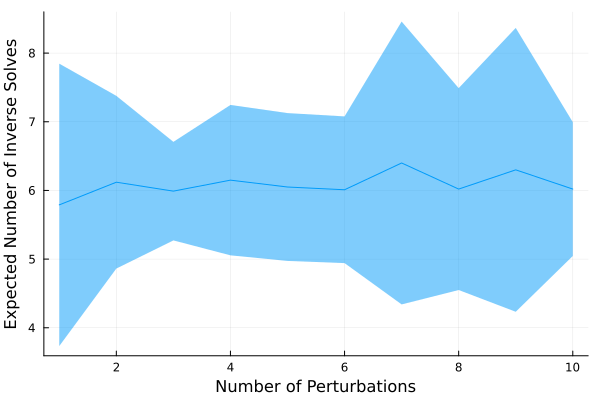
\includegraphics[width=\linewidth]{"~/partial_duality_checker/data/perturbation_iters.png"}
\caption{The number of sample points needed to converge to $\gamma_*$ to \texttt{float32} precision}
\label{fig:scaling}
\end{figure}
There is no discernable scaling of required inverse solves with the size of the system (Figure \ref{fig:scaling}) and overall the method requires no more than 3 inverse solve the vast majority of the time (Figure \ref{fig:distribution}).

\begin{figure}[H]
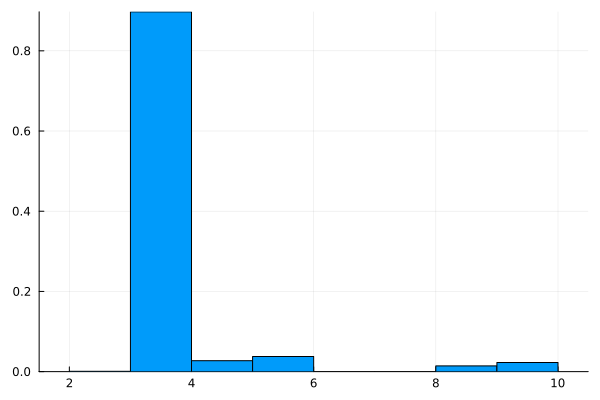
\includegraphics[width=\linewidth]{"~/partial_duality_checker/data/histogram.png"}
\caption{The distribution of number of sample points needed to converge to $\gamma_*$ to \texttt{float32} precision. This takes on average 3.3 samples with a standard deviation of 1.1.}
\label{fig:distribution}
\end{figure}

\section{Discussion}
This method's constant scaling in the number of iterations is not the whole story, as the system size increases the computational cost of sampling also increases.  The green's operator is stored in a matrix-free fashion so BiCGStab is used to compute solutions \cite{van1992bi}. A matrix-vector product here $O(n\log n)$ since GILA and for the largest system size tested here about 20 matrix-vector products are needed for each inverse solve. While a specific comparison might be imprecise as there exist different implementations of Cholesky decomposition, once one goes beyond $n$ of a few hundred it is clear that the Padé based approach is superior.

\bibliography{references}
\end{document}
